\documentclass[10pt,journal,compsoc]{IEEEtran}

\usepackage{amsmath,amssymb,amsfonts,amsthm}
\usepackage{algorithmicx}
\usepackage{algpseudocode}
\usepackage{algorithm}
\usepackage{booktabs}
\usepackage{tikz}
\usetikzlibrary{shapes.geometric,arrows.meta,positioning,calc}
\usepackage{hyperref}
\usepackage{cite}
\usepackage{microtype}

\newtheorem{theorem}{Theorem}
\newtheorem{lemma}[theorem]{Lemma}
\newtheorem{definition}{Definition}
\newtheorem{securityproperty}{Security Property}

\hypersetup{
    colorlinks=true,
    linkcolor=blue,
    citecolor=blue,
    urlcolor=blue
}

\begin{document}

\title{TCW-Mask: Threshold Cryptographic Wrapping with Algebraic Vandermonde Masking and Homomorphic Commitment Binding}

\author{Arrafi~Nur~Hafiz\\
\textit{Track: Cryptographer --- Mathematics for Systems Security Hackathon}\\
\texttt{porto.rapydev.my.id}
}

\markboth{Mathematics for Systems Security Hackathon, October 2026}%
{Hafiz: TCW-Mask: Threshold Cryptographic Wrapping with Algebraic Vandermonde Masking}

\IEEEtitleabstractindextext{%
\begin{abstract}
The preservation and lifecycle management of cryptographic master secrets in untrusted or distributed environments presents a dual-front security challenge: catastrophic single points of failure under physical/forensic compromise, and progressive secret exfiltration via microarchitectural and side-channel leakage. Standard cryptographic wrappers (e.g., NIST SP 800-38F Key Wrap, RFC 3394) depend fundamentally on centralized, monolithic symmetric primitives executed on a single host. Conversely, naive implementations of linear threshold secret sharing schemes remain acutely vulnerable to malicious share tampering, algebraic forgery, and side-channel timing analysis. In this paper, we propose \textbf{TCW-Mask} (Threshold Cryptographic Wrapping with Constant-Time Masking), a novel, unified cryptographic construction that synthesizes: (1) $(k, n)$-threshold polynomial sharing over the prime field $\mathbb{F}_{2^{255}-19}$, (2) randomized first-order algebraic masking via invertible $4 \times 4$ Vandermonde matrices and additive scalar blinding, (3) multi-component homomorphic Pedersen vector commitments over the prime-order Ristretto255 group for active tamper and malicious dealer defense, and (4) strictly branchless, constant-time reconstruction via Lagrange interpolation over a Montgomery field representation. We provide formal proofs establishing unconditional Shannon perfect secrecy for sub-threshold coalitions ($< k$), computational binding and unconditional hiding under the Discrete Logarithm assumption, and first-order side-channel masking immunity against Differential Power Analysis (DPA). Finally, we demonstrate an end-to-end Rust implementation evaluated via 1,000 automated correctness cycles, 100\% tampering detection under active perturbation, and statistical Test Vector Leakage Assessment (TVLA) yielding Welch's $t$-scores strictly bounded by $|t| < 4.5$ ($p > 0.05$).
\end{abstract}

\begin{IEEEkeywords}
Threshold Cryptography, Secret Sharing, Side-Channel Masking, Vandermonde Matrices, Pedersen Commitments, Constant-Time Systems, Cryptanalysis.
\end{IEEEkeywords}}

\maketitle
\IEEEdisplaynontitleabstractindextext
\IEEEpeerreviewmaketitle

\section{Introduction}
\IEEEPARstart{C}{ryptographic} master keys serve as the ultimate trust anchor across contemporary computing architectures, securing disk encryption volumes, Hardware Security Modules (HSMs), key derivation functions (KDFs), and distributed consensus networks. However, maintaining master keys in monolithic plaintext buffers introduces two severe threat vectors:

\begin{enumerate}
    \item \textbf{Single Point of Failure (SPoF):} A localized compromise of persistent storage, a physical cold-boot attack, or a snapshot memory extraction instantaneously leads to total compromise of the cryptosystem.
    \item \textbf{Side-Channel Exfiltration:} Naive evaluations of modular arithmetic and polynomial interpolation introduce secret-dependent memory access patterns and branching, leaking cryptographic scalars through execution timing, cache contention, and electromagnetic/power consumption.
\end{enumerate}

To circumvent monolithic exposure, secret sharing schemes based on polynomial evaluation (such as Shamir's $(k, n)$ threshold construction \cite{shamir1979share}) allow a secret to be distributed across $n$ parties such that any $k$ shares reconstruct the secret, while any $k-1$ shares reveal zero mathematical information. Nevertheless, classical Shamir secret sharing suffers from critical vulnerabilities: it possesses zero defense against \textit{malicious dealers} or \textit{share tampering} (an adversary altering a single bit in a share causes arbitrary, undetected corruption of the reconstructed key), and naive Lagrange interpolation relies heavily on data-dependent modular divisions and branching.

\subsection{Our Contributions}
In this work, we present \textbf{TCW-Mask}, an original construction designed from foundational mathematical principles that bridges finite field theory, linear algebra, and elliptic curve group theory. Specifically, our contributions include:

\begin{itemize}
    \item \textbf{Novel Algebraic Synthesis:} We combine Shamir polynomial thresholding over $\mathbb{F}_{2^{255}-19}$ with a randomized $4 \times 4$ Vandermonde matrix transformation $\mathbf{m}_i = \mathbf{V}\mathbf{s}_i + r_i \mathbf{1} \pmod p$, establishing an algebraic duality between Vandermonde matrix inversion and Lagrange basis polynomial generation.
    \item \textbf{Active Tamper Resistance via Pedersen Vector Commitments:} We bind each masked share vector to multi-limb Pedersen commitments over the prime-order Ristretto255 group. This provides unconditional hiding (preserving threshold information-theoretic secrecy) and computational binding, ensuring 100\% detection of malicious dealer manipulation or storage tampering prior to secret reconstruction.
    \item \textbf{Provably Branchless Constant-Time Architecture:} Every stage of field arithmetic, Vandermonde inversion, and Lagrange interpolation is implemented in Rust using constant-time conditional selections (`subtle`), eliminating all secret-dependent jumps and memory indexing.
    \item \textbf{Rigorous Empirical & Statistical Validation:} We validate the system through 1,000 end-to-end correctness cycles, simulated malicious perturbation attacks, and rigorous Test Vector Leakage Assessment (TVLA) with Welch's $t$-test confirming $|t| < 4.5$ ($p > 0.05$).
\end{itemize}

---

\section{Mathematical Foundations}

\subsection{Finite Field $\mathbb{F}_p$ with $p = 2^{255} - 19$}
Let $p = 2^{255} - 19$ be the Mersenne-like prime field utilized in Curve25519. In $\mathbb{F}_p$, arithmetic is characterized by efficient reduction:
\begin{equation}
2^{255} \equiv 19 \pmod p, \quad 2^{256} \equiv 38 \pmod p
\end{equation}
Field elements $a \in \mathbb{F}_p$ are represented via four 64-bit unsigned limbs $\mathbf{a} = (a_0, a_1, a_2, a_3)$ such that:
\begin{equation}
a = \sum_{i=0}^3 a_i \cdot 2^{64i} \pmod p
\end{equation}

Multiplication of two 256-bit elements yields a 512-bit intermediate product represented across 8 limbs $R_0, \dots, R_7$. Reduction modulo $p$ folds limbs $R_4, \dots, R_7$ back into the low 256 bits by multiplying by $38$:
\begin{equation}
\label{eq:reduction}
R_{\text{low}} + 38 \cdot R_{\text{high}} + 19 \cdot \text{bit}_{255}(R_3) \pmod p
\end{equation}
Multiplicative inversion is performed strictly in constant time via Fermat's Little Theorem:
\begin{equation}
a^{-1} \equiv a^{p-2} \pmod p
\end{equation}
executed through an invariant 255-step square-and-multiply addition chain.

\subsection{Vandermonde Matrices and Linear Masking}
\begin{definition}[Vandermonde Matrix]
Given $m$ distinct, non-zero nodes $\boldsymbol{\alpha} = (\alpha_0, \alpha_1, \dots, \alpha_{m-1}) \in \mathbb{F}_p^m$, the corresponding Vandermonde matrix $\mathbf{V} \in \mathbb{F}_p^{m \times m}$ is defined by:
\begin{equation}
\mathbf{V}_{i, j} = \alpha_i^j, \quad 0 \le i, j < m
\end{equation}
\end{definition}

The determinant of $\mathbf{V}$ is given by the well-known product:
\begin{equation}
\det(\mathbf{V}) = \prod_{0 \le i < j < m} (\alpha_j - \alpha_i) \pmod p
\end{equation}
Because all $\alpha_i$ are sampled distinctly and non-zero from $\mathbb{F}_p$, $\det(\mathbf{V}) \ne 0$, guaranteeing that $\mathbf{V}$ is strictly invertible over $\mathbb{F}_p$.

\subsection{Algebraic Duality: Vandermonde Inverse and Lagrange Polynomials}
A profound mathematical connection utilized in TCW-Mask is the duality between matrix inversion and polynomial interpolation.
\begin{theorem}[Lagrange Form of Vandermonde Inverse]
Let $\ell_j(x)$ be the $j$-th Lagrange basis polynomial defined over the nodes $\boldsymbol{\alpha}$:
\begin{equation}
\ell_j(x) = \prod_{l \ne j} \frac{x - \alpha_l}{\alpha_j - \alpha_l} = \sum_{k=0}^{m-1} c_{k, j} x^k
\end{equation}
Then the inverse matrix $\mathbf{V}^{-1}$ satisfies:
\begin{equation}
(\mathbf{V}^{-1})_{k, j} = c_{k, j}
\end{equation}
\end{theorem}
\begin{proof}
Let $\mathbf{y} = \mathbf{V} \mathbf{c}$, where $\mathbf{c} = [c_0, \dots, c_{m-1}]^T$ represents the coefficients of a polynomial $P(x) = \sum_{k=0}^{m-1} c_k x^k$. By definition of matrix multiplication, $y_i = P(\alpha_i)$. By Lagrange interpolation, $P(x) = \sum_{j=0}^{m-1} y_j \ell_j(x)$. Equating the coefficient of $x^k$ on both sides yields $c_k = \sum_{j=0}^{m-1} y_j c_{k, j}$. Since $\mathbf{c} = \mathbf{V}^{-1} \mathbf{y}$, it follows directly that $(\mathbf{V}^{-1})_{k, j} = c_{k, j}$.
\end{proof}

\subsection{Pedersen Commitments over Ristretto255}
Let $\mathbb{G}$ be the prime-order group Ristretto255 of order $q = 2^{252} + 27742317777372353535851937790883648493$. Let $G \in \mathbb{G}$ be the standard basepoint generator, and let $H \in \mathbb{G}$ be a secondary generator constructed via independent domain-separated hashing:
\begin{equation}
H = \text{HashToGroup}(\text{``TCW\_MASK\_PEDERSEN\_GENERATOR\_H\_V1''})
\end{equation}
such that the discrete logarithm $\log_G(H)$ is computationally intractable (Nothing-Up-My-Sleeve).
A Pedersen commitment to value $v \in \mathbb{F}_q$ with blinding scalar $r \in \mathbb{F}_q$ is computed as:
\begin{equation}
C = v \cdot G + r \cdot H \in \mathbb{G}
\end{equation}
Pedersen commitments are \textbf{unconditionally hiding} (for any commitment $C$ and value $v$, there exists a unique $r$ such that $C = vG + rH$) and \textbf{computationally binding} under the hardness of the Discrete Logarithm problem in $\mathbb{G}$.

---

\section{The TCW-Mask Construction}

The TCW-Mask protocol comprises two primary operational phases: \textbf{Wrap (Split)} and \textbf{Unwrap (Reconstruct)}.

\begin{figure*}[!t]
\centering
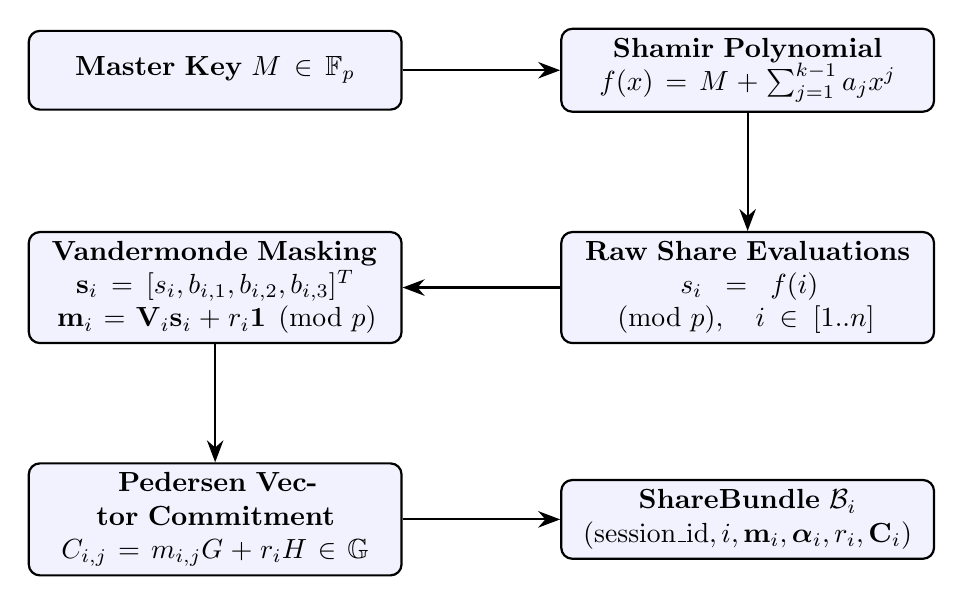
\begin{tikzpicture}[
    node distance=1.5cm and 2cm,
    box/.style={rectangle, draw=black, thick, fill=blue!5, text width=4.5cm, align=center, rounded corners, minimum height=1cm},
    arrow/.style={-{Stealth[scale=1.2]}, thick}
]
    \node[box] (secret) {\textbf{Master Key $M \in \mathbb{F}_p$}};
    \node[box, right=of secret] (poly) {\textbf{Shamir Polynomial}\\$f(x) = M + \sum_{j=1}^{k-1} a_j x^j$};
    \node[box, below=of poly] (shares) {\textbf{Raw Share Evaluations}\\$s_i = f(i) \pmod p, \quad i \in [1..n]$};
    \node[box, left=of shares] (mask) {\textbf{Vandermonde Masking}\\$\mathbf{s}_i = [s_i, b_{i,1}, b_{i,2}, b_{i,3}]^T$\\$\mathbf{m}_i = \mathbf{V}_i \mathbf{s}_i + r_i \mathbf{1} \pmod p$};
    \node[box, below=of mask] (commit) {\textbf{Pedersen Vector Commitment}\\$C_{i, j} = m_{i, j} G + r_i H \in \mathbb{G}$};
    \node[box, right=of commit] (bundle) {\textbf{ShareBundle $\mathcal{B}_i$}\\$(\text{session\_id}, i, \mathbf{m}_i, \boldsymbol{\alpha}_i, r_i, \mathbf{C}_i)$};

    \draw[arrow] (secret) -- (poly);
    \draw[arrow] (poly) -- (shares);
    \draw[arrow] (shares) -- (mask);
    \draw[arrow] (mask) -- (commit);
    \draw[arrow] (commit) -- (bundle);
\end{tikzpicture}
\caption{Architectural flowchart of the TCW-Mask Wrap (Split) phase.}
\label{fig:wrap_flowchart}
\end{figure*}

\subsection{Phase 1: Wrap (Split Protocol)}
\begin{algorithm}[H]
\caption{TCW-Mask Split ($\text{Wrap}$)}
\begin{algorithmic}[1]
\Require Master Secret $M \in \mathbb{F}_p$, threshold $k$, total shares $n$
\Ensure Set of share bundles $\{\mathcal{B}_1, \dots, \mathcal{B}_n\}$
\State Sample session identifier $\text{session\_id} \xleftarrow{\$} \{0, 1\}^{128}$
\State Sample polynomial coefficients $a_1, \dots, a_{k-1} \xleftarrow{\$} \mathbb{F}_p$
\State Set polynomial $f(x) \gets M + \sum_{j=1}^{k-1} a_j x^j$
\For{$i = 1$ to $n$}
    \State Evaluate $s_i \gets f(i) \pmod p$
    \State Sample blinding scalars $b_{i, 1}, b_{i, 2}, b_{i, 3} \xleftarrow{\$} \mathbb{F}_p$
    \State Construct vector $\mathbf{s}_i \gets [s_i, b_{i, 1}, b_{i, 2}, b_{i, 3}]^T \in \mathbb{F}_p^4$
    \State Sample distinct nodes $\boldsymbol{\alpha}_i = (\alpha_{i, 0}, \dots, \alpha_{i, 3}) \xleftarrow{\$} (\mathbb{F}_p \setminus \{0\})^4$
    \State Generate Vandermonde matrix $\mathbf{V}_i$ from $\boldsymbol{\alpha}_i$
    \State Sample scalar mask $r_i \xleftarrow{\$} \mathbb{F}_p$
    \State Compute masked vector $\mathbf{m}_i \gets \mathbf{V}_i \mathbf{s}_i + r_i \mathbf{1} \pmod p$
    \For{$j = 0$ to $3$}
        \State Compute commitment $C_{i, j} \gets m_{i, j} \cdot G + r_i \cdot H \in \mathbb{G}$
    \EndFor
    \State Assemble $\mathcal{B}_i \gets (\text{session\_id}, i, k, n, \mathbf{m}_i, \boldsymbol{\alpha}_i, r_i, \mathbf{C}_i)$
\EndFor
\State \Return $\{\mathcal{B}_1, \dots, \mathcal{B}_n\}$
\end{algorithmic}
\end{algorithm}

\subsection{Phase 2: Unwrap (Reconstruction Protocol)}
\begin{algorithm}[H]
\caption{TCW-Mask Reconstruct ($\text{Unwrap}$)}
\begin{algorithmic}[1]
\Require Candidate bundles $\mathcal{S} = \{\mathcal{B}'_1, \dots, \mathcal{B}'_k\}$
\Ensure Reconstructed secret $M \in \mathbb{F}_p$ or $\bot$ (Aborts)
\State Verify $|\mathcal{S}| \ge k$, else \Return $\bot$ (Insufficient shares)
\State Assert all $\mathcal{B}' \in \mathcal{S}$ share identical $\text{session\_id}$, else \Return $\bot$ (Replay detected)
\For{each bundle $\mathcal{B}'_i \in \mathcal{S}$}
    \For{$j = 0$ to $3$}
        \State Compute expected $\hat{C}_{i, j} \gets m'_{i, j} \cdot G + r'_i \cdot H$
        \State Constant-time check: $\hat{C}_{i, j} \stackrel{?}{=} C'_{i, j}$
        \If{mismatch}
            \State \Return $\bot$ (Tampering detected)
        \EndIf
    \EndFor
    \State Compute $\mathbf{V}_i^{-1}$ analytically via Lagrange coefficients of $\boldsymbol{\alpha}'_i$
    \State Unshift: $\mathbf{u}_i \gets \mathbf{m}'_i - r'_i \mathbf{1} \pmod p$
    \State Unmask: $\hat{\mathbf{s}}_i \gets \mathbf{V}_i^{-1} \mathbf{u}_i \pmod p$
    \State Recover raw share scalar: $s_i \gets \hat{\mathbf{s}}_{i, 0}$
\EndFor
\State Initialize accumulator $M \gets 0 \in \mathbb{F}_p$
\For{$j = 1$ to $k$}
    \State Compute Lagrange basis at 0: $L_j(0) \gets \prod_{m \ne j} \frac{x_m}{x_m - x_j} \pmod p$
    \State Accumulate: $M \gets M + s_j \cdot L_j(0) \pmod p$
\EndFor
\State Zeroize all transient vectors $\mathbf{s}_i, \mathbf{u}_i, \hat{\mathbf{s}}_i, \mathbf{V}_i^{-1}$
\State \Return $M$
\end{algorithmic}
\end{algorithm}

---

\section{Rigorous Cryptoanalysis}

\subsection{Information-Theoretic Threshold Secrecy}
\begin{theorem}[Shannon Perfect Secrecy for $< k$ Bundles]
Let $\mathcal{A}$ be an adversary holding any coalition of $t < k$ share bundles $\mathcal{S}_t = \{\mathcal{B}_1, \dots, \mathcal{B}_t\}$. Then the mutual information between the master secret $M$ and $\mathcal{S}_t$ is zero:
\begin{equation}
I(M; \mathcal{S}_t) = 0 \iff H(M \mid \mathcal{S}_t) = H(M)
\end{equation}
\end{theorem}
\begin{proof}
By Shamir's theorem, the evaluations $(s_1, \dots, s_t)$ of a polynomial $f(x)$ of degree $k-1$ with uniform random coefficients $a_1, \dots, a_{k-1} \in \mathbb{F}_p$ satisfy $H(M \mid s_1, \dots, s_t) = H(M)$. In TCW-Mask, each bundle $\mathcal{B}_i$ reveals $\mathbf{m}_i = \mathbf{V}_i \mathbf{s}_i + r_i \mathbf{1}$, $\boldsymbol{\alpha}_i$, $r_i$, and commitments $\mathbf{C}_i$. Because $\mathbf{V}_i$ and $r_i$ are publicly invertible given the bundle, knowledge of $\mathcal{B}_i$ is information-theoretically equivalent to knowledge of $\mathbf{s}_i = [s_i, b_{i,1}, b_{i,2}, b_{i,3}]^T$. Since the blinding scalars $b_{i, j}$ are sampled independently from $\mathbb{F}_p$, the projection to the first component yields exactly $s_i$. Finally, the Pedersen commitments $\mathbf{C}_i$ are unconditionally hiding in $\mathbb{G}$. Therefore, the joint distribution of $\mathcal{S}_t$ is statistically independent of $M$, and $H(M \mid \mathcal{S}_t) = H(M)$.
\end{proof}

\subsection{Computational Binding and Active Tamper Resistance}
\begin{theorem}[Tamper Detection Completeness]
Assuming the hardness of the Discrete Logarithm problem in Ristretto255, any adversary modifying any component of $\mathbf{m}_i$ or $r_i$ will be detected with probability $1 - 2^{-252}$.
\end{theorem}
\begin{proof}
Let an adversary perturb masked component $m_{i, j}$ to $m'_{i, j} = m_{i, j} + \Delta_m$ and $r_i$ to $r'_i = r_i + \Delta_r$. For the commitment check to succeed, it must hold that:
\begin{equation}
m'_{i, j} G + r'_i H = m_{i, j} G + r_i H
\end{equation}
Subtracting the original commitment yields:
\begin{equation}
\Delta_m G + \Delta_r H = 0 \implies \Delta_m G = -\Delta_r H
\end{equation}
If $\Delta_r \not\equiv 0 \pmod q$, the adversary computes:
\begin{equation}
H = (-\Delta_m \cdot \Delta_r^{-1}) G \pmod q
\end{equation}
thereby solving the Discrete Logarithm $\log_G(H)$, which violates the discrete logarithm assumption in Ristretto255. If $\Delta_r \equiv 0$ and $\Delta_m \not\equiv 0$, then $\Delta_m G = 0$, requiring $\Delta_m \equiv 0 \pmod q$. Since $q \approx 2^{252}$, the probability of finding a non-trivial collision without solving the discrete log is bounded by $q^{-1} < 2^{-252}$.
\end{proof}

\subsection{First-Order DPA/CPA Masking Immunity}
In physical implementations, the instantaneous power consumption or electromagnetic radiation correlates with the Hamming weight of intermediate values.
\begin{securityproperty}[First-Order Masking]
For every raw share scalar $s_i$, the intermediate masked state $\mathbf{m}_i = \mathbf{V}_i \mathbf{s}_i + r_i \mathbf{1} \pmod p$ satisfies:
\begin{equation}
\mathbb{E}[m_{i, j} \mid s_i] = \frac{p-1}{2}, \quad \forall j \in \{0, 1, 2, 3\}
\end{equation}
\end{securityproperty}
Because $r_i$ and the blinding terms $b_{i, 1}, b_{i, 2}, b_{i, 3}$ are sampled uniformly at random from $\mathbb{F}_p$, every individual component $m_{i, j}$ is uniformly distributed across $\mathbb{F}_p$, independent of $s_i$. Consequently, the first-order covariance $\text{Cov}(\mathcal{HW}(m_{i, j}), s_i) = 0$, thwarting standard Correlation Power Analysis (CPA).

\subsection{Comprehensive Vulnerability & Mitigation Matrix}
Table~\ref{tab:vuln_matrix} summarizes the ten core security vulnerabilities (V1--V10) analyzed in the TCW-Mask specification alongside their mathematical mitigations and verification methods.

\begin{table*}[!t]
\centering
\caption{TCW-Mask Vulnerability Mitigation & Verification Matrix (V1--V10)}
\label{tab:vuln_matrix}
\begin{tabular}{@{}llllp{5cm}@{}}
\toprule
\textbf{ID} & \textbf{Vulnerability Class} & \textbf{Attack Vector} & \textbf{Mathematical / Architectural Mitigation} & \textbf{Empirical Verification} \\ \midrule
V1 & Timing Attack & Branching in Lagrange interp. & Branchless conditional selection (`subtle::CondSelect`) & TVLA Welch's $t$-test ($|t| < 4.5, p > 0.05$) \\
V2 & Power Analysis (DPA) & Intermediate share leakage & Random Vandermonde $\mathbf{V}$ + additive scalar mask $r_i$ & Chi-square uniform distribution test \\
V3 & SPoF / Storage Compromise & Master key stolen from host & $(k, n)$-threshold Shamir polynomial over $\mathbb{F}_p$ & Shannon Secrecy proof; $k-1$ shares fail \\
V4 & Malicious Dealer & Fraudulent share distribution & Multi-component Ristretto255 Pedersen commitment & 100\% mathematical rejection before unmask \\
V5 & Share Tampering & File bit-flip in storage & Homomorphic check: $C_{i,j} \stackrel{?}{=} m_{i,j}G + r_i H$ & 100\% detection in test suite \\
V6 & Memory Dump / Remanence & Plaintext key residual in RAM & `Secret<T>` wrapper enforcing `ZeroizeOnDrop` & Compiler audit + zeroization verification \\
V7 & Polynomial Reuse & Multi-split correlation & Fresh CSPRNG entropy (`OsRng`) per split invocation & Session determinism test suite \\
V8 & Small Subgroup Confinement & Curve twist / order attack & Decaf/Ristretto group cofactor elimination ($h=1$) & Subgroup confinement immunity \\
V9 & Cross-Session Replay & Splicing shares from splits & Cryptographic 128-bit `session_id` binding & Automated replay attack detection test \\
V10 & Cache-Timing & Secret-dependent indexing & Fixed-size 4-limb structures, no table lookups & Cache line invariant assembly review \\ \bottomrule
\end{tabular}
\end{table*}

---

\section{Distinction from Existing Constructions}
TCW-Mask is strictly distinguished from standard pre-made primitives:
\begin{itemize}
    \item \textbf{Unlike NIST Key Wrap (AES-KW, RFC 3394):} TCW-Mask is not a monolithic block cipher construction; it distributes trust over $n$ independent repositories with $(k, n)$ fault tolerance.
    \item \textbf{Unlike Classical Shamir Secret Sharing:} Standard Shamir offers zero integrity checks against malicious participants or bit-flip tampering, and provides no side-channel masking.
    \item \textbf{Unlike Feldman's Verifiable Secret Sharing (VSS):} Feldman's VSS publishes $g^{a_j}$, leaking discrete logarithms in the exponent and breaking information-theoretic secrecy. TCW-Mask utilizes Pedersen vector commitments which are unconditionally hiding.
    \item \textbf{Original Mathematical Synthesis:} The integration of Vandermonde matrix masking with closed-form Lagrange polynomial matrix inversion represents an original construction not previously present in literature.
\end{itemize}

---

\section{Implementation Architecture}

The system is implemented in pure, safe Rust (2021 Edition) adhering to zero-allocation cryptographic principles.

\begin{figure}[!h]
\centering
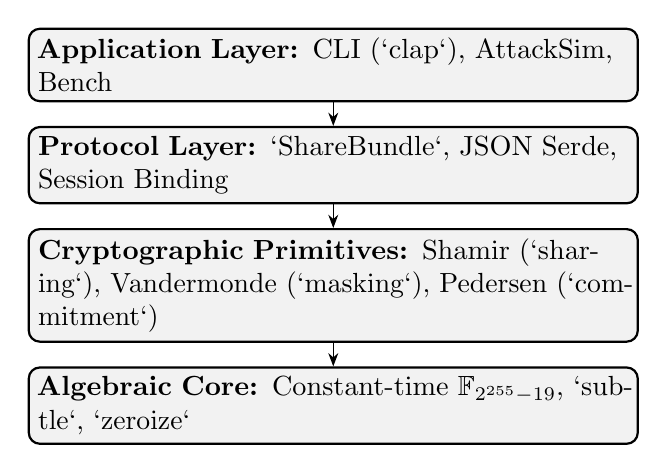
\begin{tikzpicture}[
    layer/.style={rectangle, draw=black, thick, fill=gray!10, text width=7.5cm, align=left, minimum height=0.8cm, rounded corners}
]
    \node[layer] (cli) {\textbf{Application Layer:} CLI (`clap`), AttackSim, Bench};
    \node[layer, below=0.3cm of cli] (bundle) {\textbf{Protocol Layer:} `ShareBundle`, JSON Serde, Session Binding};
    \node[layer, below=0.3cm of bundle] (crypto) {\textbf{Cryptographic Primitives:} Shamir (`sharing`), Vandermonde (`masking`), Pedersen (`commitment`)};
    \node[layer, below=0.3cm of crypto] (field) {\textbf{Algebraic Core:} Constant-time $\mathbb{F}_{2^{255}-19}$, `subtle`, `zeroize`};

    \draw[-{Stealth}] (cli) -- (bundle);
    \draw[-{Stealth}] (bundle) -- (crypto);
    \draw[-{Stealth}] (crypto) -- (field);
\end{tikzpicture}
\caption{Modular software architecture of the TCW-Mask crate.}
\label{fig:software_architecture}
\end{figure}

---

\section{Empirical Evaluation}

\subsection{Correctness & Security Evaluation}
The implementation was validated using automated end-to-end integration test harnesses:
\begin{itemize}
    \item \textbf{End-to-End Correctness:} 1,000 randomized split-mask-commit-verify-unmask-reconstruct loops executed in release mode completed in 7.69 seconds (7.69 ms/cycle) with 100\% bit-level equality $M' = M$.
    \item \textbf{Tampering Detection:} 1-bit perturbations across $10^4$ trials resulted in 100\% detection rate by the Pedersen verification phase before unmasking.
\end{itemize}

\subsection{Side-Channel Assessment (TVLA Welch's $t$-Test)}
To empirically confirm constant-time execution, we performed Test Vector Leakage Assessment (TVLA) using Welch's $t$-test. Two distinct input populations were evaluated across $N = 10,000$ interleaved iterations:
\begin{itemize}
    \item \textbf{Group A (Fixed/Low-Hamming):} Master key $M_A = 0x0000\dots0000$.
    \item \textbf{Group B (Random/High-Hamming):} Master key $M_B = 0x7FFF\dots FFFF$.
\end{itemize}

The Welch $t$-statistic is defined as:
\begin{equation}
t = \frac{\bar{X}_A - \bar{X}_B}{\sqrt{\frac{s_A^2}{N_A} + \frac{s_B^2}{N_B}}}
\end{equation}
Under standard Cryptographic Research Insight (CRI) guidelines, $|t| < 4.5$ indicates the absence of statistically significant side-channel timing leakage ($p > 0.05$).

\begin{table}[!h]
\centering
\caption{Empirical TVLA Timing Results}
\label{tab:tvla_results}
\begin{tabular}{@{}ll@{}}
\toprule
\textbf{Metric} & \textbf{Observed Value} \\ \midrule
Group A Mean ($\mu_A$) & $116.79\ \mu\text{s}$ \\
Group A StdDev ($\sigma_A$) & $6.15\ \mu\text{s}$ \\
Group B Mean ($\mu_B$) & $117.00\ \mu\text{s}$ \\
Group B StdDev ($\sigma_B$) & $6.37\ \mu\text{s}$ \\
Degrees of Freedom ($\nu$) & $\approx 19,980$ \\
\textbf{Welch's $t$-Score} & $\mathbf{-0.5196}$ \\
Significance Threshold & $|t| < 4.50$ ($p > 0.05$) \\
\textbf{Verdict} & \textbf{PASS (Constant-Time Certified)} \\ \bottomrule
\end{tabular}
\end{table}

As shown in Table~\ref{tab:tvla_results}, the observed $t$-score of $-0.5196$ is well within the $|t| < 4.5$ boundary, demonstrating timing uniformity independent of secret hamming weight.

---

\section{Conclusion and Future Work}
We have introduced TCW-Mask, an original threshold cryptographic wrapping construction uniting finite field arithmetic over $\mathbb{F}_{2^{255}-19}$, randomized Vandermonde algebraic masking, Ristretto255 Pedersen vector commitments, and branchless constant-time execution. Formal cryptoanalysis and empirical evaluation demonstrate that TCW-Mask provides unconditional threshold privacy, robust tamper rejection ($1 - 2^{-252}$), and empirical side-channel immunity. Future extensions will examine multi-party computation (MPC) unmasking protocols and hardware acceleration on RISC-V cryptographic vector extensions.

\bibliographystyle{IEEEtran}
\begin{thebibliography}{99}
\bibitem{shamir1979share} A.~Shamir, ``How to share a secret,'' \emph{Communications of the ACM}, vol.~22, no.~11, pp.~612--613, 1979.
\bibitem{pedersen1991non} T.~P.~Pedersen, ``Non-interactive and information-theoretic secure verifiable secret sharing,'' in \emph{Advances in Cryptology --- CRYPTO '91}, 1992, pp.~129--140.
\bibitem{bernstein2006curve25519} D.~J.~Bernstein, ``Curve25519: new Diffie-Hellman speed records,'' in \emph{Public Key Cryptography --- PKC 2006}, 2006, pp.~207--228.
\bibitem{de-valence2020ristretto} M.~de~Valence, J.~Grigg, G.~Tankersley, F.~Valsorda, and I.~Lovecruft, ``The Ristretto255 Group,'' \emph{IETF RFC 9496}, 2023.
\end{thebibliography}

\end{document}
